\subsection{Giraph}
Giraph is a graph processing framework, inspired by Pregel, initially developed at Yahoo!. It has since become an Apache Incubator project\footnote{\url{http://incubator.apache.org/giraph/}}. Giraph is still under development, with more features being added and improved.

\subsubsection{Pregel}
Pregel is a framework developed at Google for large-scale graph processing. The purpose of Pregel was to produce a scalable and fault-tolerant platform with an API that is sufficiently flexible to express arbitrary graph algorithms \cite{pregel}. Existing solutions, other than Pregel, which achieve large-scale graph processing do suffer from issues ranging from poor performance, to a lack of fault tolerance within the system. Pregel addresses these issues within its framework.

A Pregel program executes as a series of parallel supersteps, similar in style to the Bulk Synchronous Parallel computation model described in \cite{bsp}. At each superstep, each active vertex performs some computation, which could modify the state of itself, its outgoing edges or send messages to other vertices to be received in the next superstep. An active vertex can also $VoteToHalt$, which stops this vertex it from performing any extra computation whilst the algorithm is being executed, unless the inactive vertex receives a message, in which case it becomes active again to process the messages it has received. When all vertices have voted to halt, the algorithm terminates.

\begin{figure}[htbp]
  \centering
    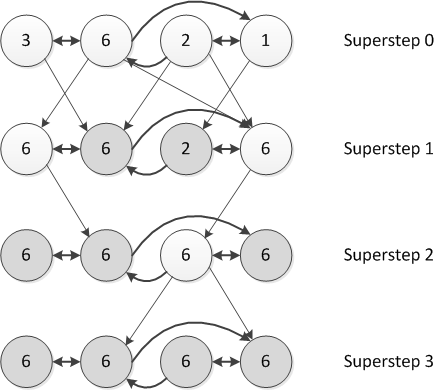
\includegraphics[width=0.5\textwidth]{./img/superstep}
  \caption{Maximum Value Example. Lighter lines are messages. Shaded vertices have voted to halt \cite{pregel}.}
  \label{fig:superstep}
\end{figure}

Figure \ref{fig:superstep} shows an example program in Pregel, which finds the maximum vertex value. Initially, all vertices are active, and send a message to each vertex they are connected directly containing their value. In the next superstep, if a vertex receives a message with a higher value than its currently stored value, then it stores the new higher value, otherwise the vertex deactivates as it currently has a local maximum whilst the program has not terminated. The vertices which did change send their value send a message containing their updated value to their neighbours. In superstep 2, the third vertex activates and changes its value from 2 to 6 as it receives a message containing the value 6. The two active vertices deactivate because they did not receive a message. The third vertex then sends a message to the second and fourth vertices containing the value 6, and in the third superstep, no vertex receiving a message changes its value, so does not need to send a message resulting in all vertices becoming inactive and terminating the program. The maximum value of all the vertices within the graph is now stored in all vertices.

As a Pregel program begins execution, multiple copies of the program start executing on a cluster of machines. A single copy is assigned as the $master$ which does not perform any work for the actual program, and instead manages the remaining $worker$ copies of the program. The $master$ partitions the input graph across the $workers$ and instructs the $workers$ to perform a superstep. This causes one iteration of the program to occur, and is repeated until all vertices vote-to-halt. The $master$ can the instruct each $worker$ to save its partition of the graph to memory.

The use of an underlying Bulk Synchonous Parallel model provides the Pregel framework with a simple way to model iteration of graph algorithms, and also provides a simple way to achieve a fault tolerant system. Each superstep in the execution of a Pregel program provides a natural barrier to synchronise each vertex's computation. If a $worker$ fails to communicate with the $master$ within a defined time period, the $master$ assumes that the $worker$ has failed, and can restart the program from the checkpoint made at the previous superstep completion, re-partitioning the graph if the failed $worker$ is still unavailable.

The Pregel framework also provides some extra useful features called combiners and aggregators. A combiner groups together a series of messages from one vertex to another into a single message containing the result of an operation on these messages. This is to reduce the overhead incurred from sending many messages and then performing the same operation at the receiving vertex. An aggregator is a global data construct, which each vertex has access to its value at each superstep, and the value can be updated at the end of each superstep in time for the next superstep. Aggregators can be used to store information about a graph, such as the number of edges in the graph.

Pregel also supports mutations of the graph an algorithm is being executed on. There are two types of mutations, global and local. A global mutation includes the addition and removal of vertices, as these can affect more that just a single vertex. Global mutations are partially ordered, and the effects of these mutations are seen in the next superstep. A local mutation includes a single vertex adding or removing an edge to another vertex. As these only affect the vertex which is performing these mutations, they happen immediately without any conflicts.

\lstset{language=C++,caption={PageRank algorithm in Pregel \cite{pregel}},label=lst:pregelpagerank,tabsize=2,breaklines=true,breakatwhitespace=true,frame=single}
\begin{lstlisting}[float]
class PageRankVertex
			: public Vertex<double, void, double> {
	public :	
		virtual void Compute(MessageIterator* msgs) {
			if (superstep() >= 1) {
				double sum = 0;
				for(; !msgs->Done(); msgs->Next())
					sum += msgs->Value();
				*MutableValue() = 0.15 / NumVertices() + 0.85 * sum;
			}
			
			if (superstep() < 30) {
				const int64 n = GetOutEdgeIterator().size();
				SendMessageToAllNeighbors(GetValue() / n);
			} else {
				VoteToHalt();
			}
		}
};					
\end{lstlisting} 

Listing \ref{lst:pregelpagerank} shows how the PageRank algorithm \cite{pagerank} can be written using the Pregel framework. It can clearly be seen how the algorithm works. Each vertex receives a series of messages which contain the PageRank for the vertex which sent the message. The sum of these PageRanks is then computed, and the damping factor applied, and the result is stored as the value of the vertex. This values is then divided by the number of outgoing edges from the vertex, and is then sent as a message to each of the vertices the vertex is connected to.

\subsubsection{Giraph}
Giraph is a framework which was designed for large-scale graph processing on Hadoop. There are a number of existing solutions to achieve large-scale graph processing, however these also have their own problems.

Graph algorithms can be executed as a sequence of map-reduce jobs in Hadoop, but this suffers from the overheads of repeatedly launching these jobs and the map-reduce model is not a good fit for graph algorithms. Pregel itself has problems in that it requires a separate computing infrastructure, and is also unavailable to non-Google employees. The Message Passage Interface can also be used for graph processing, however it lacks any form of fault tolerance and is consider too generic \cite{giraphtalk}.

\lstset{language=Java,caption={PageRank algorithm in Giraph \cite{giraphtalk}},label=lst:giraphpagerank,tabsize=2,breaklines=true,breakatwhitespace=true,frame=single}
\begin{lstlisting}[float]
public class SimplePageRankVertex extends HadoopVertex<LongWritable, DoubleWritable, FloatWritable, DoubleWritable> {

	public void compute(Iterator<DoubleWritable> msgIterator) {
		double sum = 0;
		
		while (msgIterator.hasNext()) {
			sum += msgIterator.next().get();
		}
		
		setVertexValue(new DoubleWritable((0.15f/getNumVertices()) + 0.85f * sum);
		
		if (getSuperstep() < 30) {
			long edges = getOutEdgeIterator().size();
			
			sendMsgToAllEdges(new DoubleWritable(getVertexValue().get() / edges));
		} else {
			voteToHalt();
		}
	}
}					
\end{lstlisting}

Listing \ref{lst:giraphpagerank} shows the PageRank algorithm \cite{pagerank} produced using Giraph. Strong comparisons can be seen between this, and the Pregel implementation in Listing \ref{lst:pregelpagerank}. Both Listings show that a vertex receives a series of messages, of which the values of each are summer together. A damping factor is then applied and the result stored as the value of the vertex, before this value divided by the number of outgoing edges is sent to each vertex this vertex is connected to.

Small differences can be seen, due to Giraph using Hadoop as an underlying component, such as the type system used in Giraph being composed from Java objects as opposed to primitive date types in Pregel.